\section{Theoretical and Conceptual Framework}
\label{sec:theoreticalframework}

\begin{figure}[h] % h stands for 'here'
    \centering
    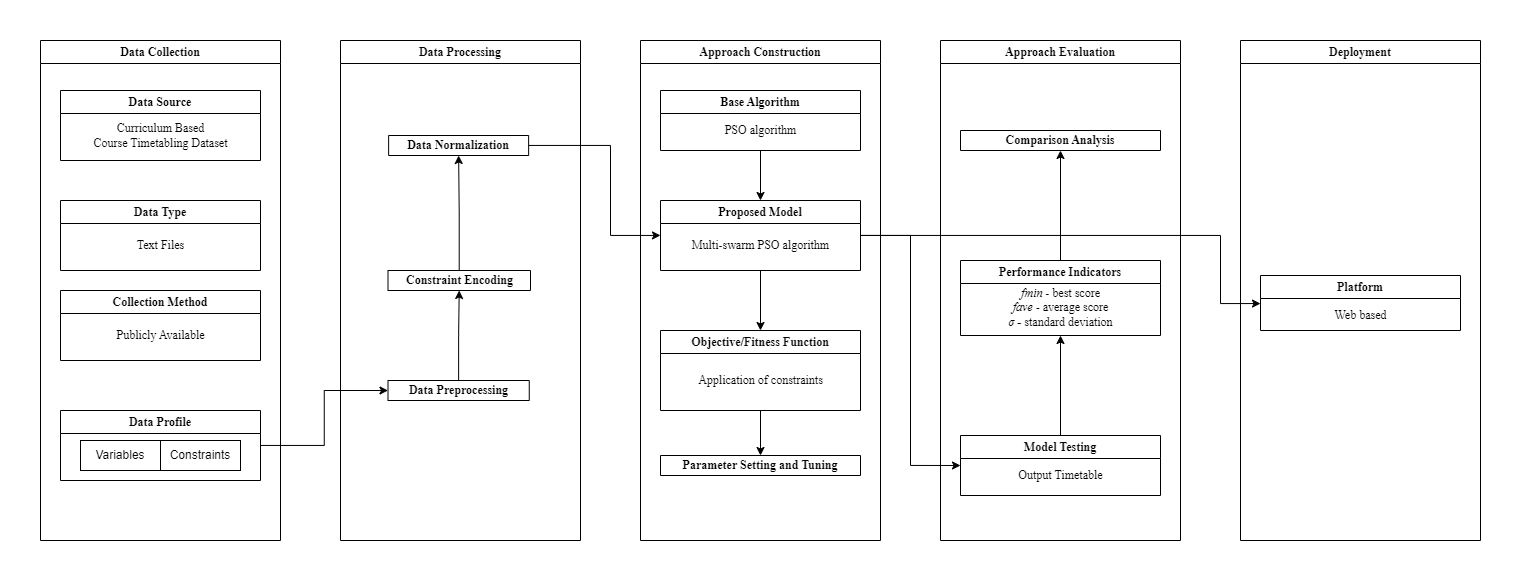
\includegraphics[width=1\textwidth]{framework}
    \caption{Theoretical and Conceptual Framework}
    \label{fig:framework} % label for referencing
\end{figure}

The theoretical and conceptual framework of this study comprises five interconnected components: Data Collection, Data Processing, Approach Construction, Approach Evaluation, and Deployment. Benchmark datasets are collected, cleaned, and preprocessed to ensure reliable and standardized inputs for optimization. The multi-swarm optimization model is then constructed and parameterized to address problem-specific requirements. Its performance is assessed by the degree to which it satisfies objectives and improved through adjustment to maximize effectiveness. The solution is finally deployed using a web-based interface where users can upload problem instances and get real-time optimized outputs.